%!TEX root = spadini_davide.tex

\chapter{Gossip-based Aggregation}
\label{cha:aggregation}
To complete our analysis, we implemented a gossip-based aggregation protocol on top of our \ac{WPSS}, in order to actually test our peer sampling service in a real peer-to-peer application. Aggregation is a common name for a set of functions that provide a summary of some global system property. In other words, they allow local access to global information in order to simplify the task of controlling, monitoring and optimization in distributed applications. Examples of aggregation functions include network size, total free storage, maximum load, average uptime, location and intensity of hotspots, etc.~\cite{aggregation}. 

The core of the protocol is a simple gossip-based communication scheme in which each node periodically selects some other random node to communicate with. During this communication the nodes update their local approximate values by performing some computation based on their previous approximate values. This local pairwise interaction is designed in such a way that all approximate values in the system will quickly converge to the desired aggregate value. 

\section{Gossip-based Aggregation algorithm}
We consider the same network of the tests, consisting of a large collection of nodes that are assigned unique identifiers and that communicate through message exchanges. 

We assume that each node in the network holds a numeric value and we want to calculate the average among the nodes. In a practical setting, this value can characterize any aspect of the node or its environment (e.g., the load at the node, available storage space, temperature measured by a sensor network, etc.). The task of the protocol is to continuously provide all nodes with an up-to-date estimate of an aggregate function, computed over the values held by the current set of nodes. The algorithm is taken from~\cite{aggregation} and it is shown in \textbf{Algorithm 2}.

\begin{algorithm}[H]
  \SetKwProg{Upon}{upon receive}{ do}{end}
  \SetKwProg{Every}{every}{ do}{end}
  \SetKwProg{Init}{init}{ do}{end}

  \Init{}{
  	$s_p = random()$
  }

  \Every{$\delta$}{
  	$q \leftarrow \getNeighbour$\;
  	send $s_p$ to \textit{q}\;
  	$s_q \leftarrow \textsf{\textit{receive}}(q)$\;
  	$s_p ← \update(s_p,s_q)$\;
  }

  \Upon{$receive(s_q)$}{
   	send $s_p$ to q\;
    $s_p ← \update(s_p,s_q)$\;
  }

 \caption{Push-pull gossip protocol executed by node \textit{p}. The local state of \textit{p} is denoted as $s_p$.}
\end{algorithm}

The algorithm runs on all the peers and it contains one timer and one event-handler. Every $\delta$ time the node initiates an information exchange with a random neighbour \textit{q} by sending it a message containing the local state $s_p$ and waiting for a response with the remote state $s_q$. The other function instead waits for messages sent by an initiator and replies with the local state. The term push-pull refers to the fact that each information exchange is performed in a symmetric manner: both participants send and receive their states.

We also have two other methods: the \getNeighbour and the \update. The first one returns a random node from the view of \textit{p}, this function uses the underlying peer sampling service that we implemented before. The \update function instead computes a new local state based on the current local state and the remote state received during the information exchange. The output of \update depends on the specific aggregation function being implemented by the protocol. In this section, we limit the discussion to computing the average over the set of numbers distributed among the nodes, so the implementation will be $(s_p + s_q) / 2$. 

The \init function initializes the local value of the node. We test two different implementations of this method: 
\begin{enumerate}
	\item all the nodes start with a random value between 0 and 1. The expected output is the average over all these local values.
	\item one node starts with 1 and the others with 0. The expected output is $1/N$, and if we do the inverse we obtain the total number of nodes present in the network (\textbf{Counting protocol}).
\end{enumerate}

As we can notice, in every round of the algorithm each node pushes its local value to a random node present in the network, and it waits to respond to other requests. What we expect is that, after few cycles, all the nodes converge to the same value. 

\section{Evaluation}
\label{sec:evaluation_aggregation}
We now evaluate the implementation described above, that is built on our peer sampling service, in other words using the \getNeighbour function over the view obtained from the \ac{WPSS}. The environment is the same as in the previous tests:
\begin{itemize}
	\item $N = 1000$ nodes
	\item $\delta = 1s$
	\item all the nodes join following a Poisson distribution with a mean inter-arrival time of 100 milliseconds
\end{itemize}

For the \ac{WPSS} we set $\Delta = 1000$ and the view size equals to 50. 

In Fig.~\ref{fig:aggregation_average} is represented the average among all the nodes and also the minimum and maximum values. As we can see in the first rounds the average is varying, and the maximum and minimum values are quite higher. After some rounds, the average stabilizes to the right value while the minimum and maximum values converge quickly to 0. At round 15 all the nodes have the same value with an accuracy of at least 4 decimal place. 

In Fig.~\ref{fig:aggregation_standard_deviation} we can see that the standard deviation decreases every round following an exponential distribution. This is expected, because the difference between the maximum and minimum decreases exponentially and after as few as 20 cycles the initial difference is reduced by several orders of magnitude. This means that after a small number of cycles all nodes will possess very accurate estimates of the global average.

\begin{figure}[p]
\centering
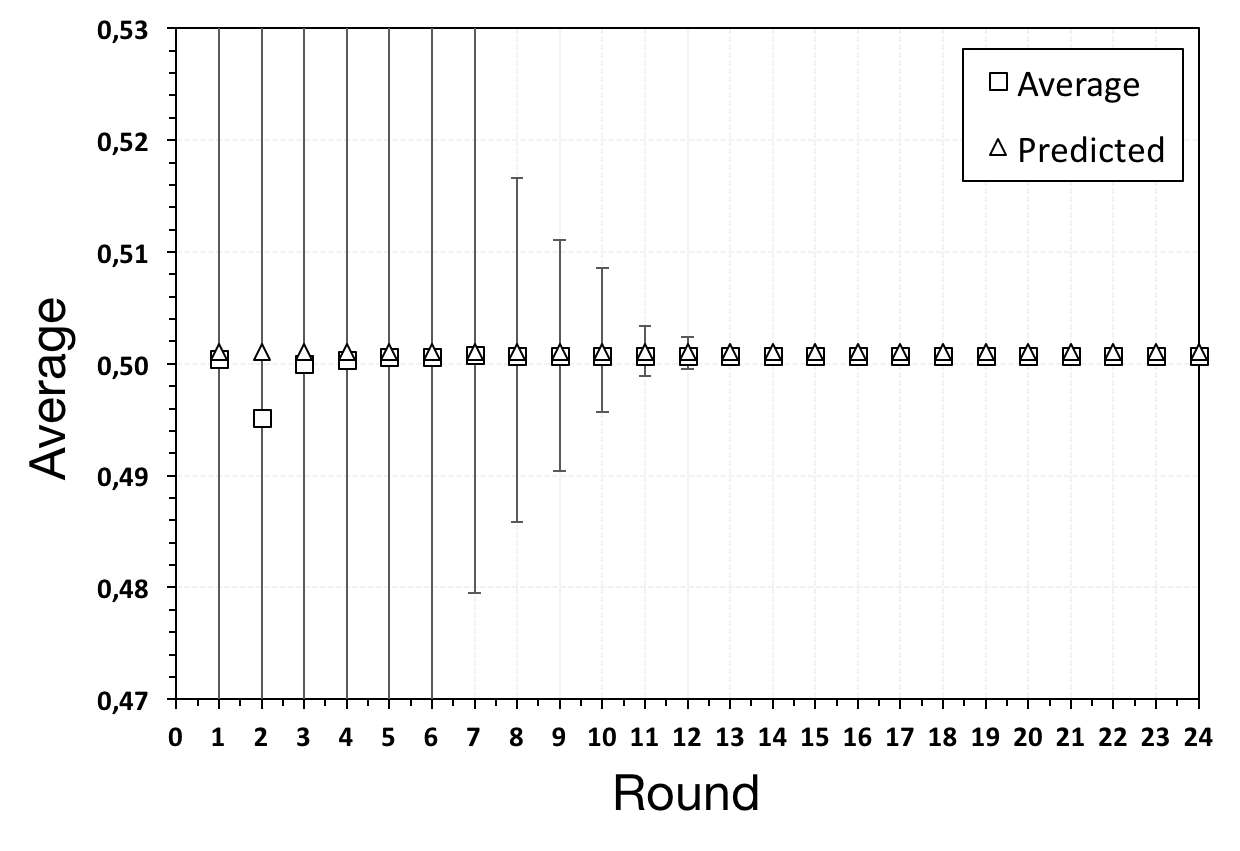
\includegraphics[keepaspectratio=true, width=0.8\textwidth]{images/aggregation_average}
\caption{Average evolution with error bars.}
\label{fig:aggregation_average}
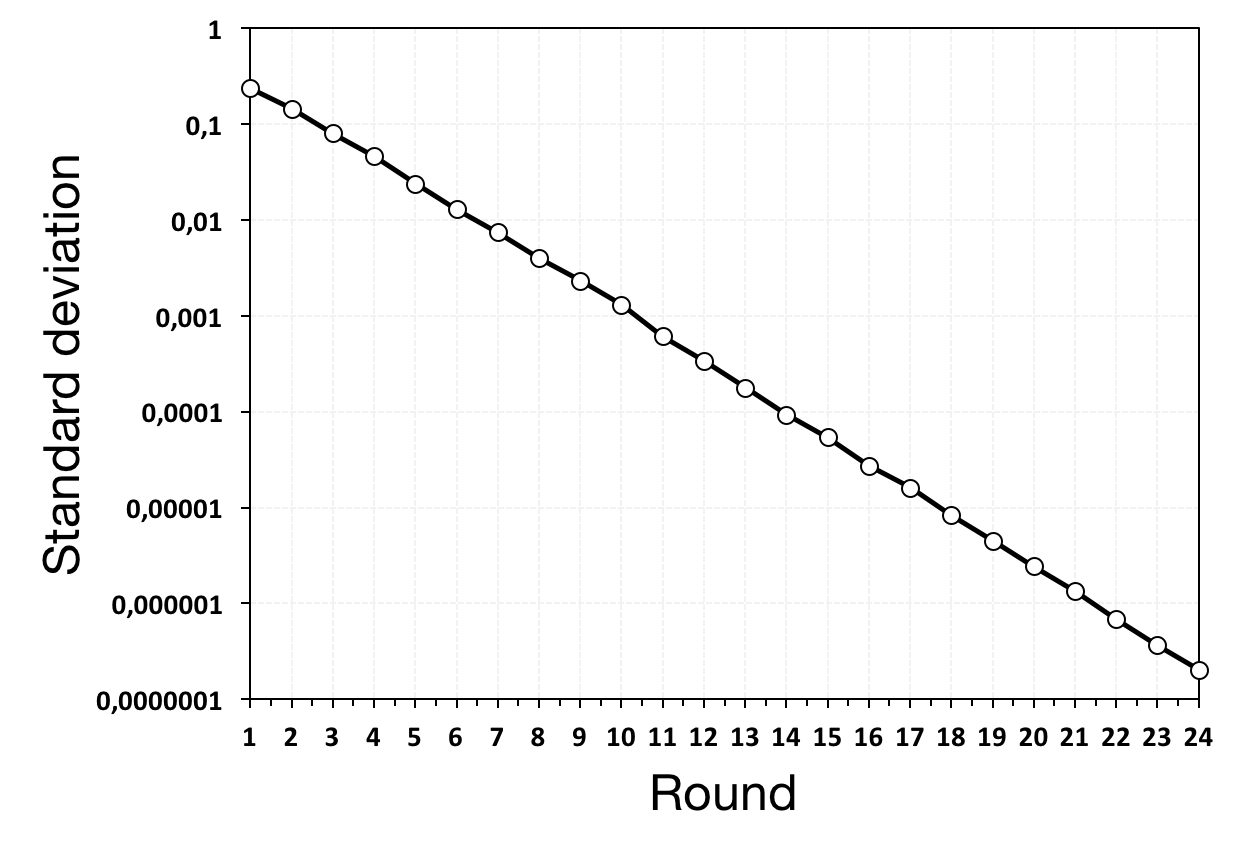
\includegraphics[keepaspectratio=true, width=0.8\textwidth]{images/aggregation_standard_deviation}
\caption{Standard deviation evolution.}
\label{fig:aggregation_standard_deviation}
\end{figure}

In Fig.~\ref{fig:aggregation_conv_factor} we calculate the convergence factor, using the formula $\sigma_i^2 / \sigma_{i-1}^2$, and we compare it with the theoretically predicted convergence factors shown in~\cite{aggregation}, which is $1 / 2\sqrt{e}$. As we can notice it confirms the predicted result, following the dotted gray line, so at each round of algorithm the standard deviation decreases by 30\%.

\begin{figure}[ht]
  \centering
  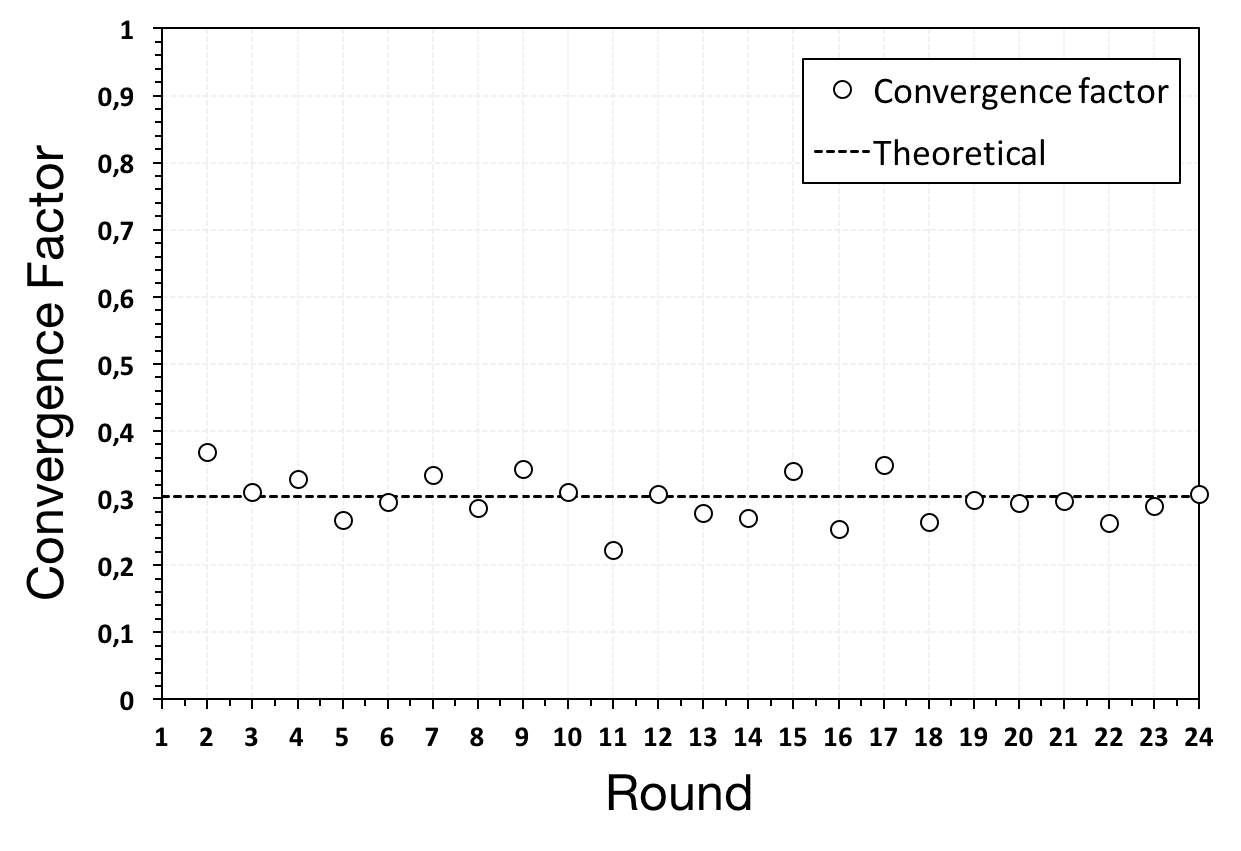
\includegraphics[keepaspectratio=true, width=0.8\textwidth]{images/aggregation_conv_factor}\caption{Convergence factor $\sigma_i^2 / \sigma_{i-1}^2$ evolution.}
  \label{fig:aggregation_conv_factor}
\end{figure}


\newpage
We now evaluate the aggregation protocol with a different initial case in which only one node will start with a value equals to 1 and all the others start with 0. What we expect is to obtain, after few cycles, an average equals to $1/N$ on all the nodes. Remind that we have $N = 1000$.

In Fig.~\ref{fig:counting_average} we represent the average among all the nodes and also the minimum and maximum values. As we can notice, in the first rounds the average is not well defined and it is fluctuating, since a lot of nodes will exchange messages with values equals to 0, and few of them will reach the node that has a correct average. However, after few rounds the average converges to the correct value and also the minimum and maximum converge to 0. With $N = 1000$, the predicted average is $1 / 1000 = 0.001$ and the experimented value that we obtained is 0.00100140314042.

In Fig.~\ref{fig:counting_standard_deviation} we represent the standard deviation evolution and as we can see it behaves similarly, at the beginning the standard deviation is high and then it follows an exponential distribution. In Fig.~\ref{fig:counting_conv_factor} we calculate the convergence factor, using the same formula as before. As we can notice until the $14^{th}$ round a lot of noise is present, and then it converges to the theoretical value as in the previous case.

\begin{figure}[p]
\centering
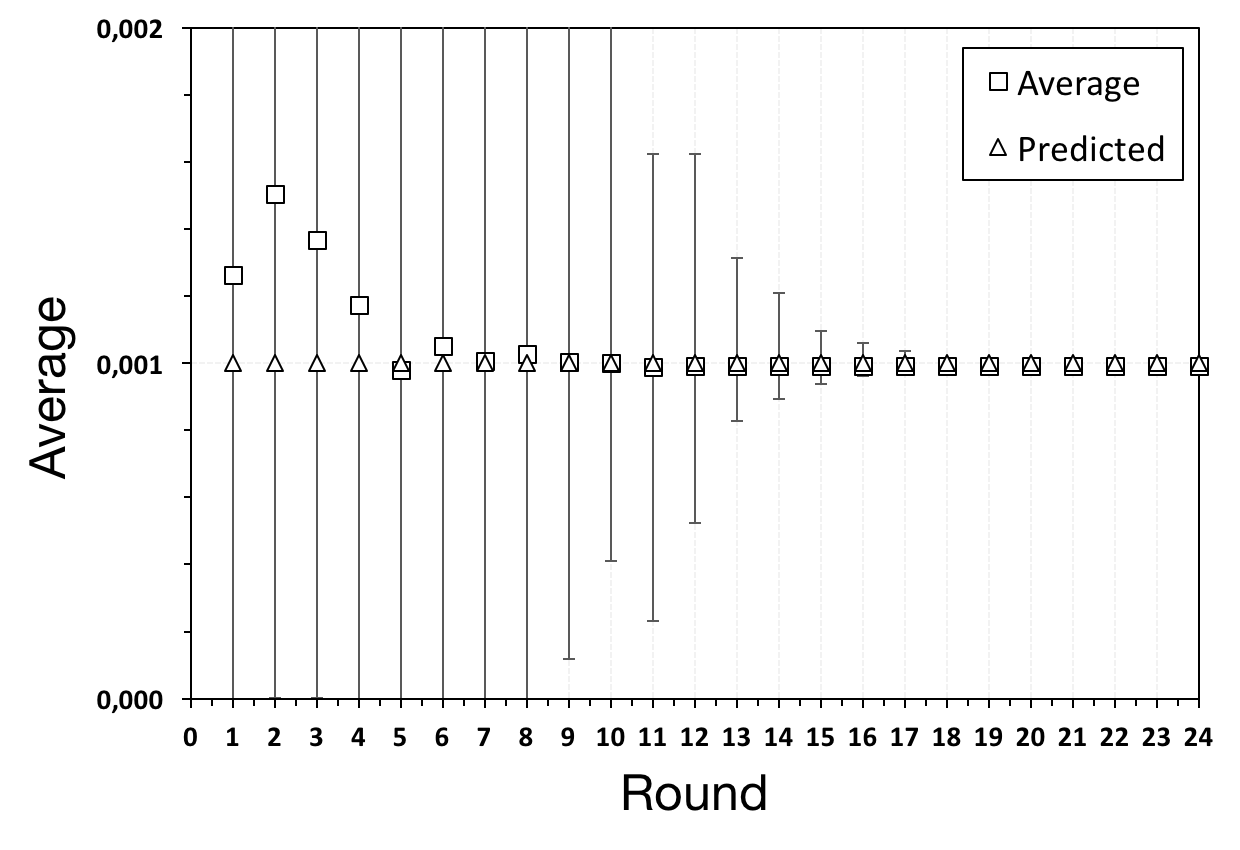
\includegraphics[keepaspectratio=true, width=0.8\textwidth]{images/counting_average}
\caption{Average evolution with error bars.}
\label{fig:counting_average}
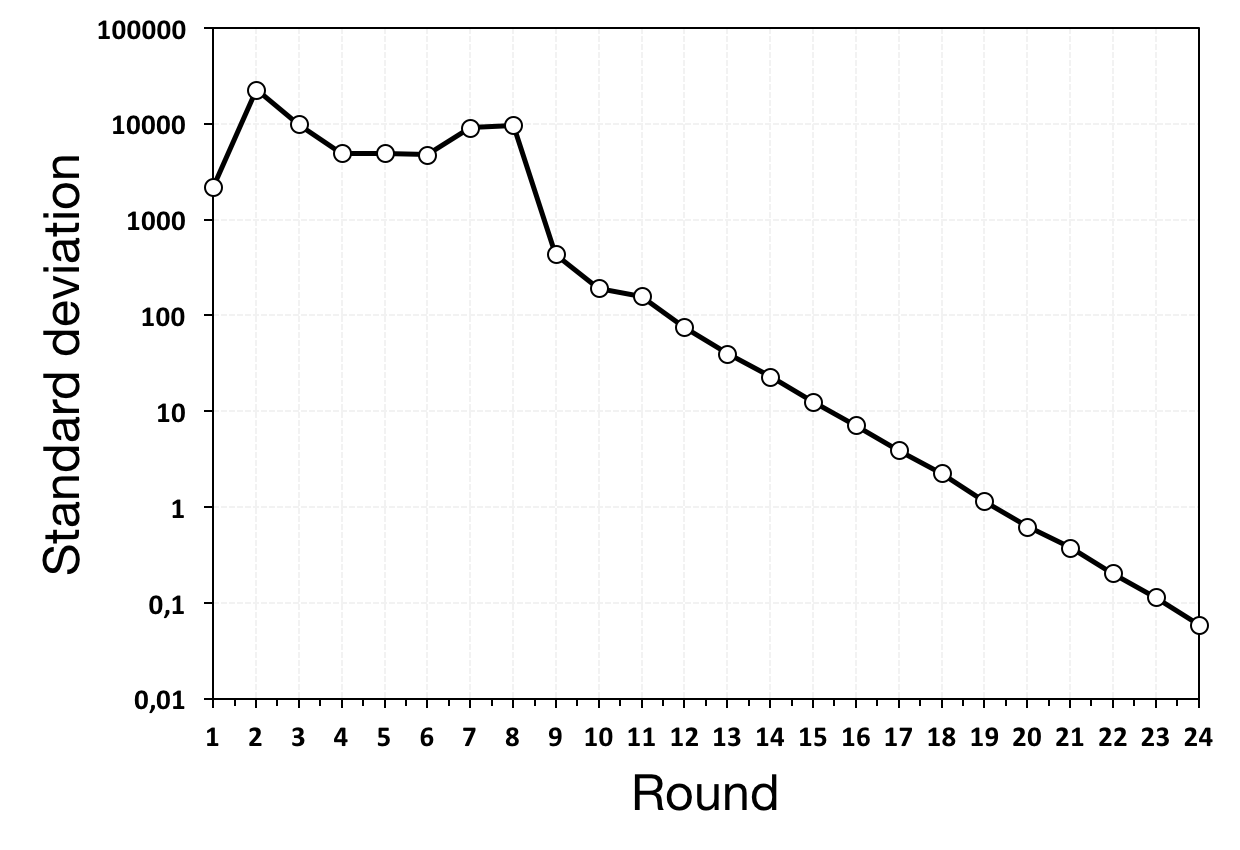
\includegraphics[keepaspectratio=true, width=0.8\textwidth]{images/counting_standard_deviation}
\caption{Standard deviation evolution.}
\label{fig:counting_standard_deviation}
\end{figure}


\begin{figure}[ht]
  \centering
  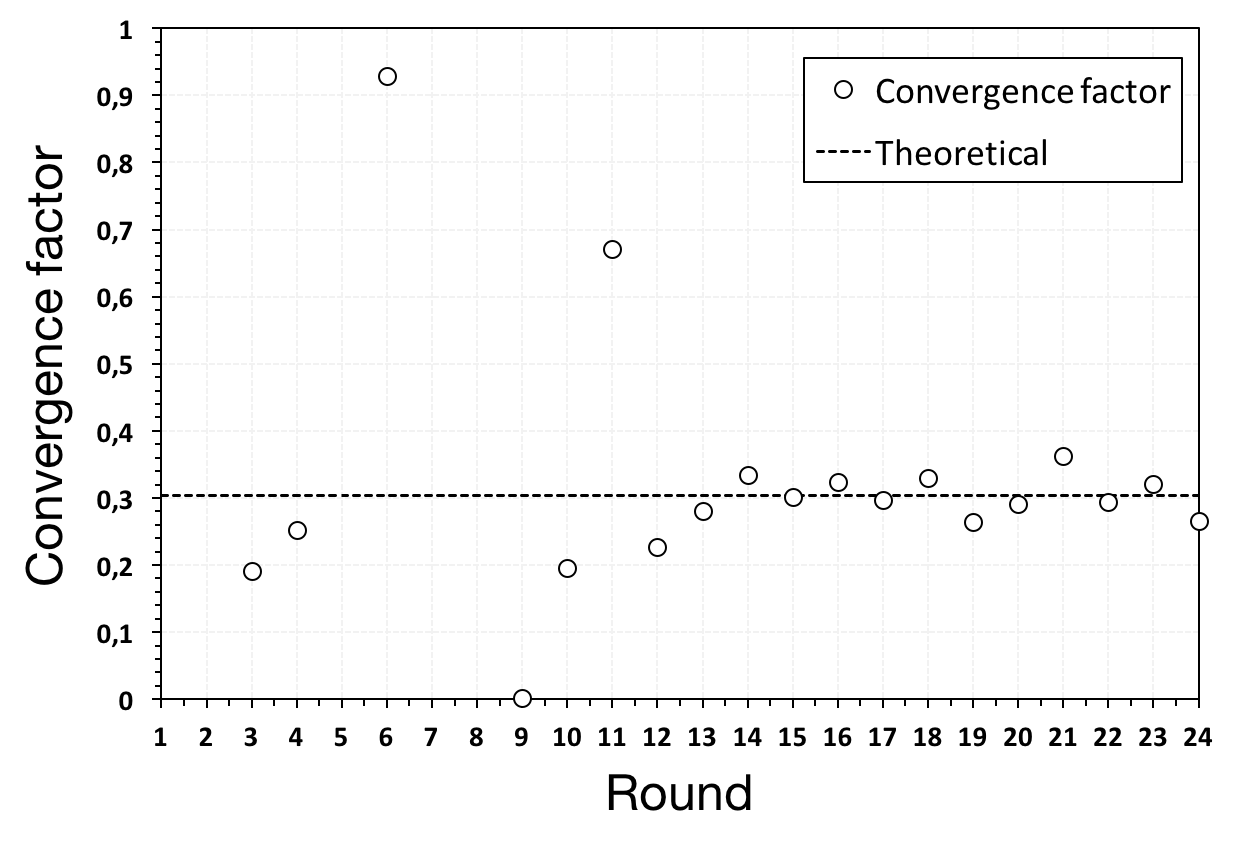
\includegraphics[keepaspectratio=true, width=0.8\textwidth]{images/counting_conv_factor}\caption{Convergence factor $\sigma_i^2 / \sigma_{i-1}^2$ evolution.}
  \label{fig:counting_conv_factor}
\end{figure}
